\documentclass[10pt]{article}
\usepackage[OE]{express}
\providecommand{\e}[1]{\ensuremath{\times 10^{#1}}} 
\providecommand{\mb}[1]{\mathbf{#1}}
\providecommand{\mh}[1]{\mathbf{\hat{#1}}}
\providecommand{\bs}[1]{\boldsymbol{#1}} 
\providecommand{\intinf}{\int_{-\infty}^{\infty}}


\begin{document}
\title{Single-Molecule Orientation Determination With Polarized Illumination:
  Modeling and Microscope Design Comparison}

\author{Talon Chandler,\authormark{1,*} Shalin Mehta,\authormark{2} Rudolf Oldenbourg,\authormark{2, 3} and Patrick J. La Rivi\`ere\authormark{1}}

\address{\authormark{1}University of Chicago, Department of Radiology, Chicago, IL, USA.\\
\authormark{2}Marine Biological Laboratory, Bell Center for Regenerative Medicine, Woods Hole, MA, USA.\\
\authormark{3}Brown University, Department of Physics, Providence, RI, USA.}
\email{*talonchandler@talonchandler.com} %% email address is required

%%%%%%%%%%%%%%%%%%% abstract and OCIS codes %%%%%%%%%%%%%%%%
\begin{abstract*}
  TODO
\end{abstract*}

\ocis{(180.0180) Microscopy; (260.5430) Polarization; (110.0110) Imaging systems; (180.2520) Fluorescence microscopy; (180.6900) Three-dimensional microscopy.}  

%%%%%%%%%%%%%%%%%%%%%%% References %%%%%%%%%%%%%%%%%%%%%%%%%
%% Comment before submission
\bibliography{paper}
\bibliographystyle{osajnl}

%% Copy .bbl and uncomment these before submission
% \begin{thebibliography}{99}
% \bibitem{gallo99} K. Gallo and G. Assanto, ``All-optical diode based on second-harmonic generation in an asymmetric waveguide,'' \josab {\bfseries 16}(2), 267--269 (1999).
% \end{thebibliography}

\section{Introduction}
TODO:
  \begin{itemize}
  \item General paragraph about the dipole orientation imaging.
  \item Current state of the art: scanning, detection polarization modulation,
    geometries
  \item We propose single-molecule orientation determination with polarized
    illumination. Compare with others. Highly parallel imaging for live cells.
  \item Section by section summary. 
  \end{itemize}
% Single molecule orientation determination is important because

% A variety of techniques have been tested to determine the orientation of
% single molecules:

% polarized detection [Fourkas], shape analysis [Moerner], other things from
% Moerner review. 

% We propose polarized illumination as an complementary method to polarized
% detection. We get the speed (no shape analysis required). We don't waste any
% dose (polarized light throws away light dose). 

% In this work we make three contributions:
% \begin{itemize}
% \item we develop the polarized illumination forward model for a broad class of
%   microscopes (section 2.X-2.X)
% \item we develop metrics to compare the performance of polarized illumination
%   microscopes 
% \item we use these metrics to compare microscopes design and make recommendations
%   for polarized illumination microscopes. 
% \end{itemize}

\section{Methods}
In this section we will develop a method to compare polarized illumination
microscope designs. In sections \ref{excitation}--\ref{forward} we develop the
forward model for single-frame microscopes with a fixed illumination and
detection orientation. In section \ref{designs} we list a variety of ways that
single-frame microscopes can be combined to create experimentally realizable
multi-frame microscopes. Finally, in section \ref{metrics} we develop metrics
that we will use to compare multi-frame microscopes.

\subsection{Excitation Efficiency}\label{excitation}
Consider polarized K\"ohler illumination incident on a single fluorophore at the
focal point with the optical axis aligned along the $\mh{z}$ axis. In this section we
will calculate the \emph{excitation efficiency} in this geometry---the fraction
of the incident power that excites the fluorophore.

We start with the unit electric field transmitted by the polarizer,
\begin{align}
 \hat{\mb{E}}_{\text{exc}} = \cos\phi_{\text{exc}}\hat{\mb{x}} +
\sin\phi_{\text{exc}}\hat{\mb{y}},\label{eq:excfield}
\end{align}
where $\phi_{\text{exc}}$ is the angle between the transmission axis of the
excitation polarizer and the $\mh{x}$ axis. Next, we model the action of the
illumination lens by multiplying the electric field vector by a position
dependent rotation matrix,
  \begin{align}
  \mb{R}(\mh{r}) &= \begin{bmatrix} \cos\theta\cos^2\phi + \sin^2\phi & (\cos\theta -1)\sin\phi\cos\phi & -\sin\theta\cos\phi\\ (\cos\theta - 1)\sin\phi\cos\phi & \cos\theta\sin^2\phi + \cos^2\phi & -\sin\theta\sin\phi \\ \sin\theta\cos\phi& \sin\theta\sin\phi & \cos\theta \end{bmatrix}
  \end{align}
  where
  \begin{align}
   \hat{\mb{r}} = \sin\theta\cos\phi\hat{\mb{x}} + \sin\theta\sin\phi\hat{\mb{y}} + \cos\theta\hat{\mb{z}} 
  \end{align}
  is a unit vector that points from the origin to the point where the incident
  electric field intersects the Gaussian sphere of the condenser lens. Next, we
  find the power that excites the fluorophore by taking the dot product of the
  rotated incident field $\mb{R}(\mh{r})\mh{E}_{\text{exc}}$ and the excitation
  dipole moment
\begin{align}
  \hat{\bs{\mu}}_{\text{exc}} = \sin\Theta\cos\Phi\hat{\mb{x}} + \sin\Theta\sin\Phi\hat{\mb{y}} + \cos\Theta\hat{\mb{z}}
\end{align}
then taking its modulus squared. If the incident fields are spatially incoherent
then we can find the total power that excites the fluorophore by integrating over the
illuminated region of the Gaussian sphere $\Omega$ where
\begin{align}
  \Omega &= \{(\phi, \theta)\ |\ \phi \in (0,2\pi], \theta\in [0, \alpha]\} \\
  \alpha &= \arcsin\left(\frac{\text{NA}}{n}\right). \label{eq:alpha}
\end{align}

Finally, we find the fraction of the incident power that excites the fluorophore by
dividing the total excitation power by the total incident power. The complete expression for the excitation efficiency in vector notation is 
\begin{align}
  \eta_{\text{exc}} = \frac{\int_{\Omega}d\mh{r}|\hat{\bs{\mu}}_{\text{exc}}\cdot\mb{R}(\mh{r})\mh{E}_{\text{exc}}|^2}{\int_{\Omega}d\mh{r}}\label{eq:exc}. 
\end{align}

We can substitute equations \ref{eq:excfield}--\ref{eq:alpha} into equation
\ref{eq:exc} and simplify to express the excitation efficiency in scalar notation as
\begin{align}
  \eta_{\text{exc}} &= D\{A + B\sin^{2}{\Theta} + C\sin^{2}{\Theta} \cos{[2 (\Phi - \phi_{\text{exc}}})]\}\label{eq:scalarexc}
\end{align}
where
\begin{subequations}
\begin{align}
  A &= \frac{1}{4} - \frac{3}{8} \cos{\alpha } + \frac{1}{8} \cos^{3}{\alpha }\\
  B &= \frac{3}{16} \cos{\alpha } - \frac{3}{16} \cos^{3}{\alpha }\\
  C &= \frac{7}{32} - \frac{3}{32} \cos{\alpha } - \frac{3}{32} \cos^{2}{\alpha } - \frac{1}{32} \cos^{3}{\alpha}\\
  D &= \frac{4}{3(1 - \cos\alpha)}.
\end{align}\label{eq:coefficients}%
\end{subequations}

At the beginning of this section we assumed that the fluorophore was located at
the focal point of the condenser. If the condenser is aplanatic then we can
relax this assumption and the above expressions are valid for fluorophores anywhere
in the focal plane.

We also assumed that we are using incoherent K\"ohler illumination. If we
illuminate the back aperture with a weakly focused laser beam and scan the laser
beam slowly compared to the coherence time of the laser, the fluorophore will be
excited as if it were excited by a single plane wave. Therefore, we can find the
excitation efficiency of weakly focused scanned laser illumination by taking the
limit of equation \ref{eq:scalarexc} as $\alpha \rightarrow 0$ which gives
\begin{align*}
  \eta_{\text{exc}} &= \sin^2\Theta\cos^2(\Phi - \phi_{\text{exc}}).
\end{align*}

\subsection{Detection Efficiency}\label{detection}
Fourkas calculated the detection efficiency of a single fluorophore when an
objective with a polarizer is aligned along the $\mh{z}$ axis
\cite{fourkas2001}. We use his expressions to calculate the detection efficiency
without a polarizer as
\begin{align}
  \eta_{\text{det}} = 2(A + B\sin^2\Theta). \label{eq:scalardet}
\end{align}
Note that the detection efficiency only depends on $\Theta$, not $\Phi$, because
there is no detection polarizer. Also note that $A$ and $B$ in equation
\ref{eq:coefficients} are a factor of $\frac{3}{2}$ larger than the expressions
given by Fourkas. We found that Fourkas' expressions were incorrectly
normalized, and the extra factor of $\frac{3}{2}$ corrects the error.

\subsection{Oblique Illumination and Detection}\label{oblique}
In sections \ref{excitation} and \ref{detection} we assumed that both the
illumination and detection objectives had $\mh{z}$ aligned optical axes. To extend
the forward model to oblique optical axes, we express the dipole orientation in
rotated coordinates using the following expressions
\begin{align}
    \theta' &= \arccos\left(\sin\psi\cos\Phi\sin\theta + \cos\psi\cos\theta\right)\label{eq:thetap}\\
  \Phi' &=
          \begin{cases}
            \arccos\left(\frac{\cos\psi\cos\Phi\sin\theta - \sin\psi\cos\theta}{\sqrt{1 - (\sin\psi\cos\Phi\sin\theta + \cos\psi\cos\theta)^2}}\right) \ \ \ &0 \leq \Phi < \pi  \\
            -\arccos\left(\frac{\cos\psi\cos\Phi\sin\theta - \sin\psi\cos\theta}{\sqrt{1 - (\sin\psi\cos\Phi\sin\theta + \cos\psi\cos\theta)^2}}\right) \ \ \ &-\pi \leq \Phi < 0\\
          \end{cases}
\end{align}
where $\psi$ is the angle that the optical axis makes with the $\mh{z}$ axis in
the $\mh{x}$ direction. 

\subsection{Single-Frame Microscopes}\label{forward}
The detected intensity is the product of the excitation efficiency, the
detection efficiency, and the total intensity emitted by the fluorophore if the
excitation and detection efficiency were 1 
\begin{align}
  I = I_{\text{tot}}\eta_{\text{exc}}\eta_{\text{det}}\label{eq:forward_frame}.
\end{align}
Equation \ref{eq:forward_frame} is the forward model for a \emph{single-frame
  microscope}. Figure \ref{fig:single-frame} shows three representative examples of
single frame microscopes. 

\begin{figure}[htbp]
\centering\includegraphics[width=\textwidth]{single-frame}
\caption{Representative examples of single-frame microscopes.\newline \newline
  \textbf{Columns left to right:} 1) schematics of single-frame microscopes
  where the solid line encloses the illumination solid angle, the dashed line
  encloses the detection solid angle, and the arrow indicates the transmission
  axis of the illumination polarizer; 2) the excitation efficiency, see equation
  \ref{eq:scalarexc}; 3) the detection efficiency, see equation
  \ref{eq:scalardet}; (4) the total efficiency, the product of the detection and
  excitation efficiencies.\newline \newline \textbf{Rows top to bottom:} 1)
  epi-illumination (NA = 1.1) with $x$-polarized light and epi-detection (NA =
  1.1); 2) orthogonal illumination (NA = 0.8) and detection (NA = 0.8); 3)
  oblique illumination (NA = 0.8) and detection (NA = 0.8).}
  \label{fig:single-frame}
\end{figure}

The intensity measured by a single-frame microscope does not give us enough
information to reconstruct the 3D orientation of a single fluorophore. Next, we
will consider combining several single-frame microscopes to create
\emph{multi-frame microscopes.}

\subsection{Multi-Frame Microscopes}\label{designs}
One way to collect multiple frames is to add a universal compensator to the
illumination arm and rapidly select the incident polarization by changin
$\phi_{\text{exc}}$ \cite{oldenbourg1995}. All of the multi-frame microscopes we
will consider in this paper use a universal compensator with four polarization
settings separated by 45${}^{\circ}$.

We also consider designs that use extra detection and illumination arms. Wu et
al. have implemented a microscope that uses orthogonal objectives that can act
as both illumination and detection arms \cite{wu2013}. Wu et al. has also added
a third view to their microscopes to further improve resolution
\cite{wu2016}. We will explore the possibility of using these geometries for
orientation determination of fluorophores.

\subsection{Evaluation Metrics}\label{metrics}
Our goal is to evaluate the ability of a microscope design to estimate the
parameters $\Theta$ and $\Phi$ from intensity data. 

For each microscope design and fluorophore orientation we calculate the Fisher
information matrix. If the intensity is Poisson distributed the
Fisher information matrix is given by
\begin{align}
  \mb{F} &= \sum_{k=1}^N \frac{1}{I_k}
  \begin{bmatrix}
    \frac{\partial I_k}{\partial \Theta}\frac{\partial I_k}{\partial \Theta}&\frac{\partial I_k}{\partial \Theta}\frac{\partial I_k}{\partial \Phi}\\\\
    \frac{\partial I_k}{\partial \Theta}\frac{\partial I_k}{\partial \Phi}&\frac{\partial I_k}{\partial \Phi}\frac{\partial I_k}{\partial \Phi}\\    
  \end{bmatrix}
\end{align}
where $I_k$ is the forward model for the $k$th frame of an $N$ frame microscope. 

A common way to evaluate the ability to estimate the parameters $\Theta$ and
$\Phi$ from the data is to calculate the Cramer-Rao lower bound (CRLB) for each
parameter \cite{kay1993}. The CRLBs are given by the diagonal elements of the
inverse of the Fisher information matrix and they give the minimum variance of
unbiased estimators for each parameter. Some authors use the product of the
CRLBs multiplied by the Jacobian determinant to find the area of uncertainty in
parameter space \cite{agrawal2012}.

CRLBs and the associated area of uncertainty are parametrization dependent---if
we choose a different coordinate system then the values will change
significantly. We would like to compare microscope designs without choosing a
parametrization.

Instead of the taking the product of the CRLBs, we use
\begin{align}
  \sigma_{\Omega} &= \sin\Theta\sqrt{\text{det}\{\mb{F}^{-1}\}}
\end{align}
as our evaluation metric. We take the determinant of the inverse Fisher
information matrix---a parametrization independent value often called the
\emph{generalized variance} \cite{anderson1958}---take the square root, then
multiply by the Jacobian determinant, $\sin\Theta$. We call $\sigma_{\Omega}$ the
\emph{solid-angle uncertainty} because it has units of steradians and is a
measure of the uncertainty of the orientation parameters.

We calculated $\sigma_{\Omega}$ on 100,000 approximately equally spaced points
on the unit sphere for each microscope design. A desirable microscope design
will have a small solid-angle uncertainty that is uniform for all fluorophore
orientations. To summarize and compare microscope designs we use the median and
median absolute deviation (MAD) of the solid-angle uncertainty.

\section{Results}
\subsection{One-Arm Designs}\label{one-arm}
\begin{itemize}
\item Figure \ref{fig:single-arm} shows the results when we used a single
  objective to illuminate and detect.
\item We swept through the illumination and detection NA while keeping the
  incident power ($I_{\text{tot}}$) constant and found that the lowest median and
  MAD of the solid-angle uncertainty occurs with a small
  illumination NA and a large detection NA.
\item A small illumination NA maximizes the ``contrast'' in the excitation
  efficiency, while a large detection NA maximizes the ``contrast'' in the
  detection efficiency.
\end{itemize}

\begin{figure}[htbp]
\centering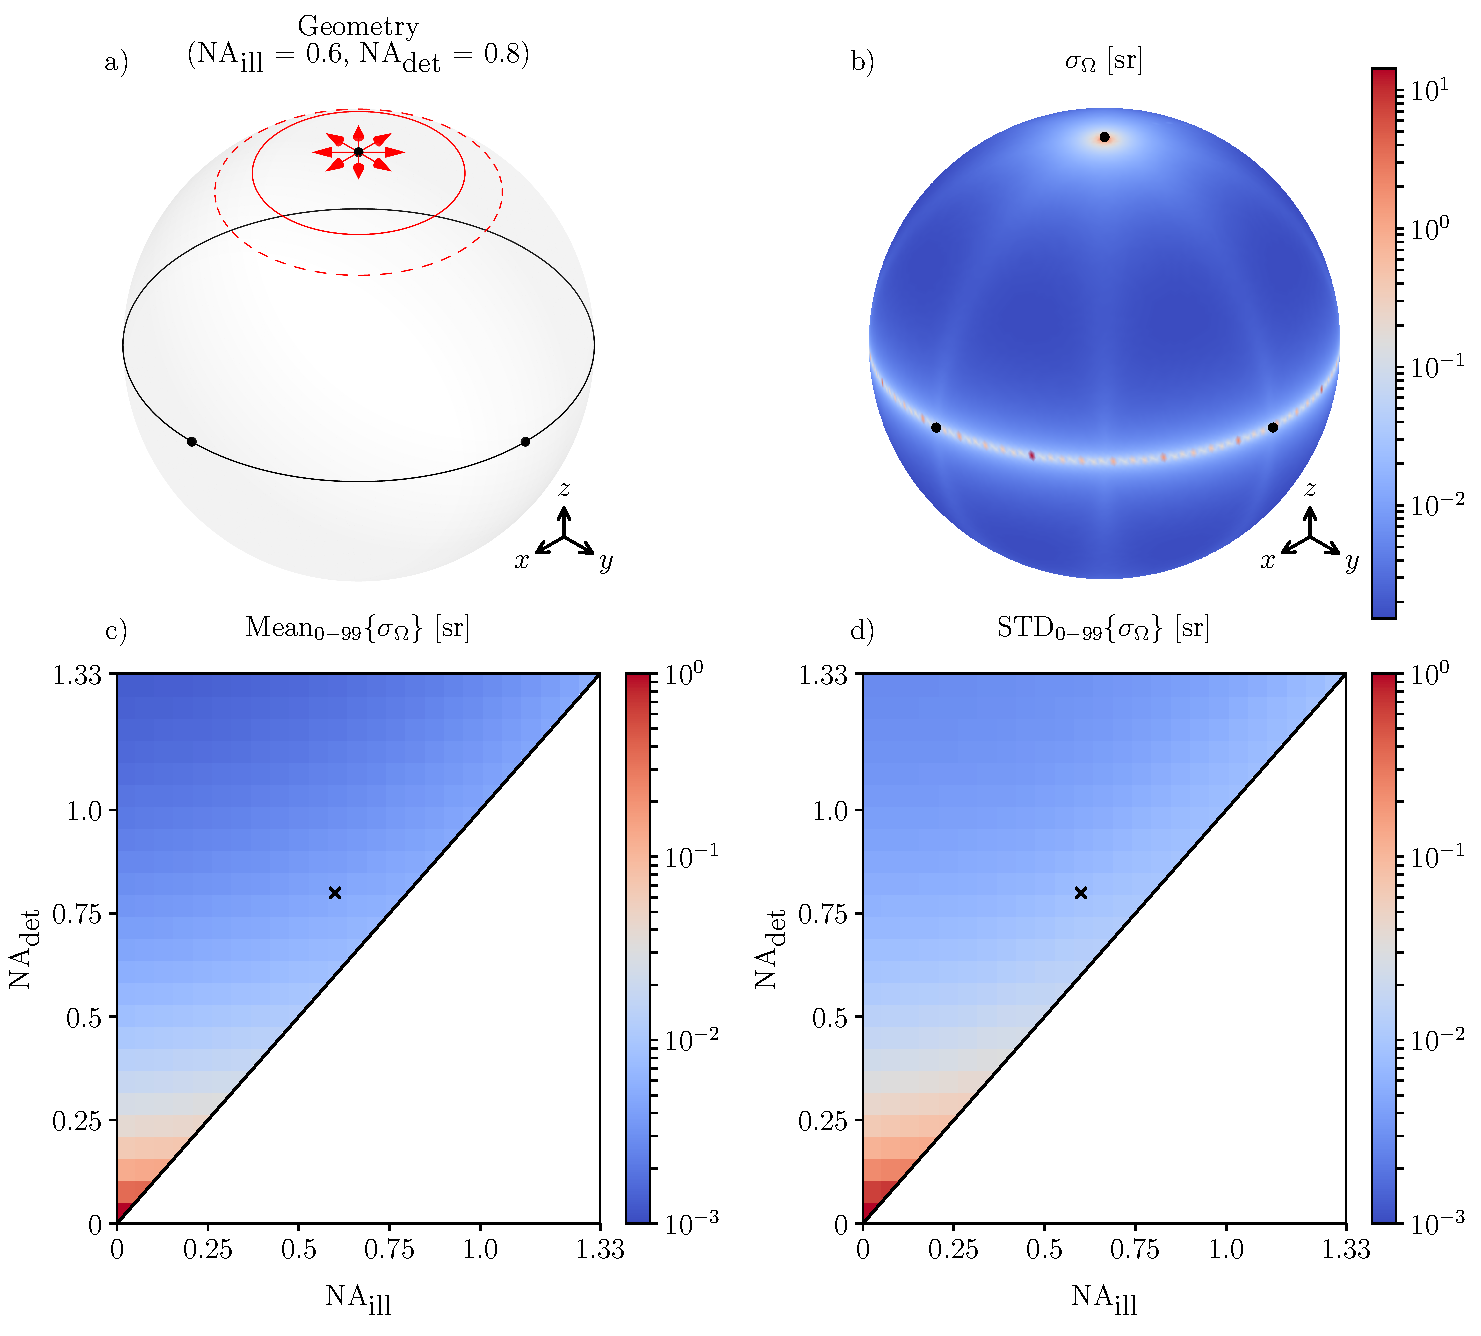
\includegraphics[width=\textwidth]{single-arm}
\caption{Epi-illumination microscope with varying NA and underfilling of the
  back aperture. a) Schematic of a single-arm four-frame epi-illumination
  microscope. b) Solid angle uncertainty for the microscope in a) when
  $I_{\text{tot}} = 1000$ photons. c) Median of the solid-angle uncertainty as a
  function of illumination and detection NA. d) MAD of solid-angle uncertainty
  as a function of illumination and detection NA. The microscope in a) and b) is
  indicated by a cross in c) and d).}
\label{fig:single-arm}
\end{figure}

\subsection{Two-Arm Designs}
\begin{itemize}
\item Figure \ref{fig:symmetric-widefield} shows the results when we used a
  symmetric widefield design. Both objectives serve as a an illumination and
  detection NA.
\item We swept through the NA and the angle between the objectives while
  considering steric constraints and while keeping the incident power constant.
  We found that the lowest median of the solid-angle uncertainty occurs the largest
  possible NA. We also found the increasing NA always lowers the MAD, but orthogonal
  arms are not always best. At large NA, it is advantageous to move the objectives
  as close or as far apart within steric constraints. 
\end{itemize}

\begin{figure}[htbp]
\centering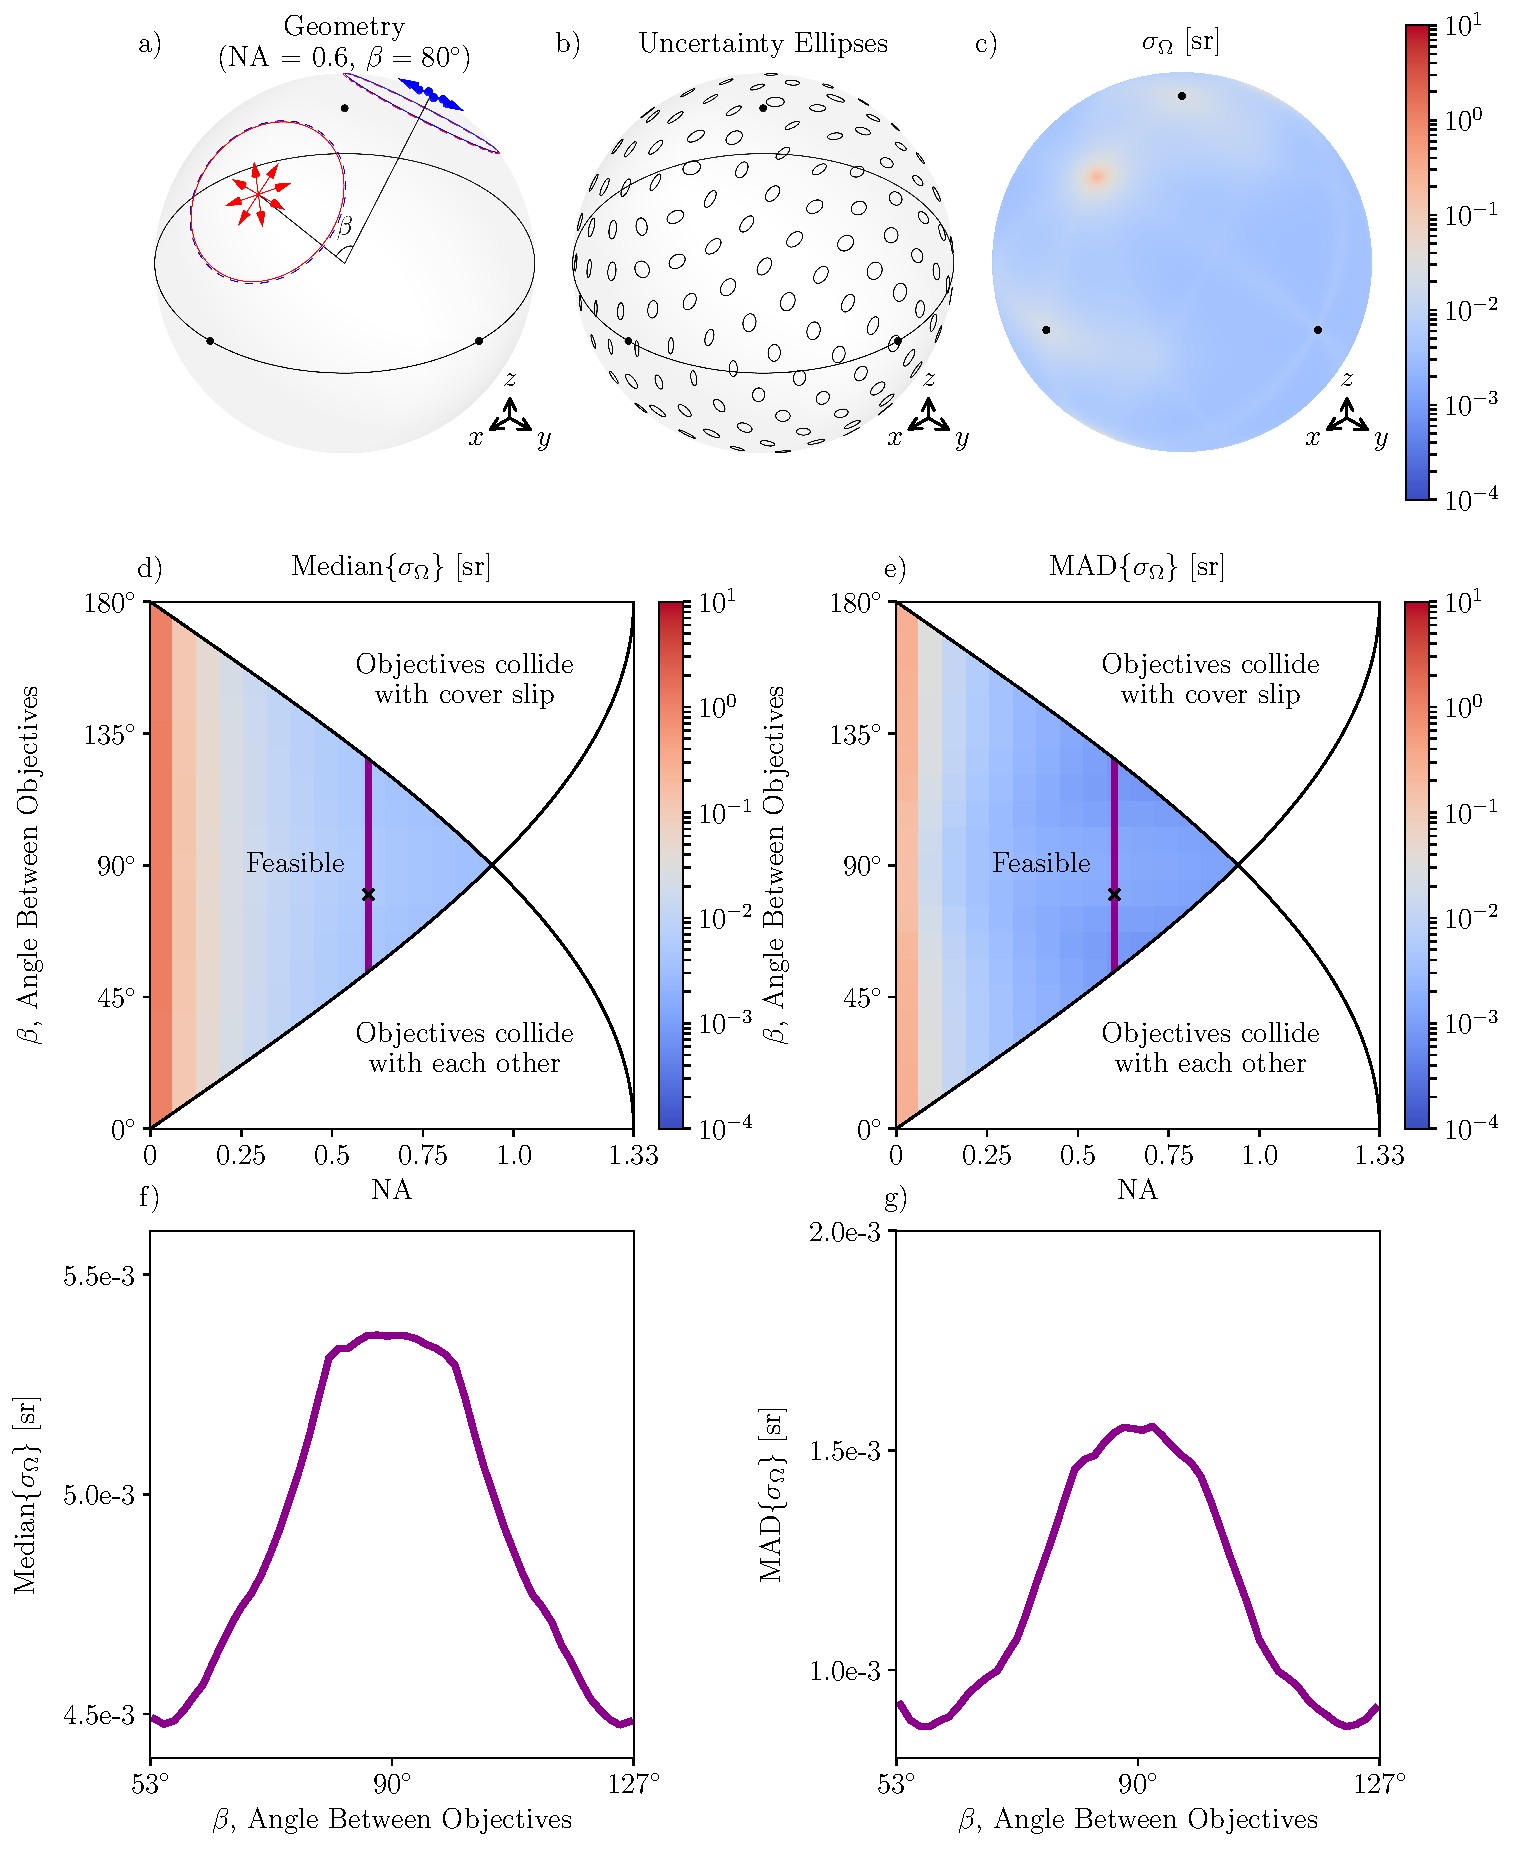
\includegraphics[width=\textwidth]{symmetric-widefield}
\caption{Symmetric widefield designs with varying NA and angle between objectives. See the Fig. \ref{fig:single-arm} caption for an explanation of a)-d).}
\label{fig:symmetric-widefield}
\end{figure}

\begin{itemize}
\item Figure \ref{fig:double-arm} shows the results when we used a
  symmetric widefield design and varied the illumination and detection NA. 
\item Similar to section \ref{one-arm}, we found that the best microscopes occur
  with a large detection NA and a small illumination NA (like light sheet illumination).
\end{itemize}

\begin{figure}[htbp]
\centering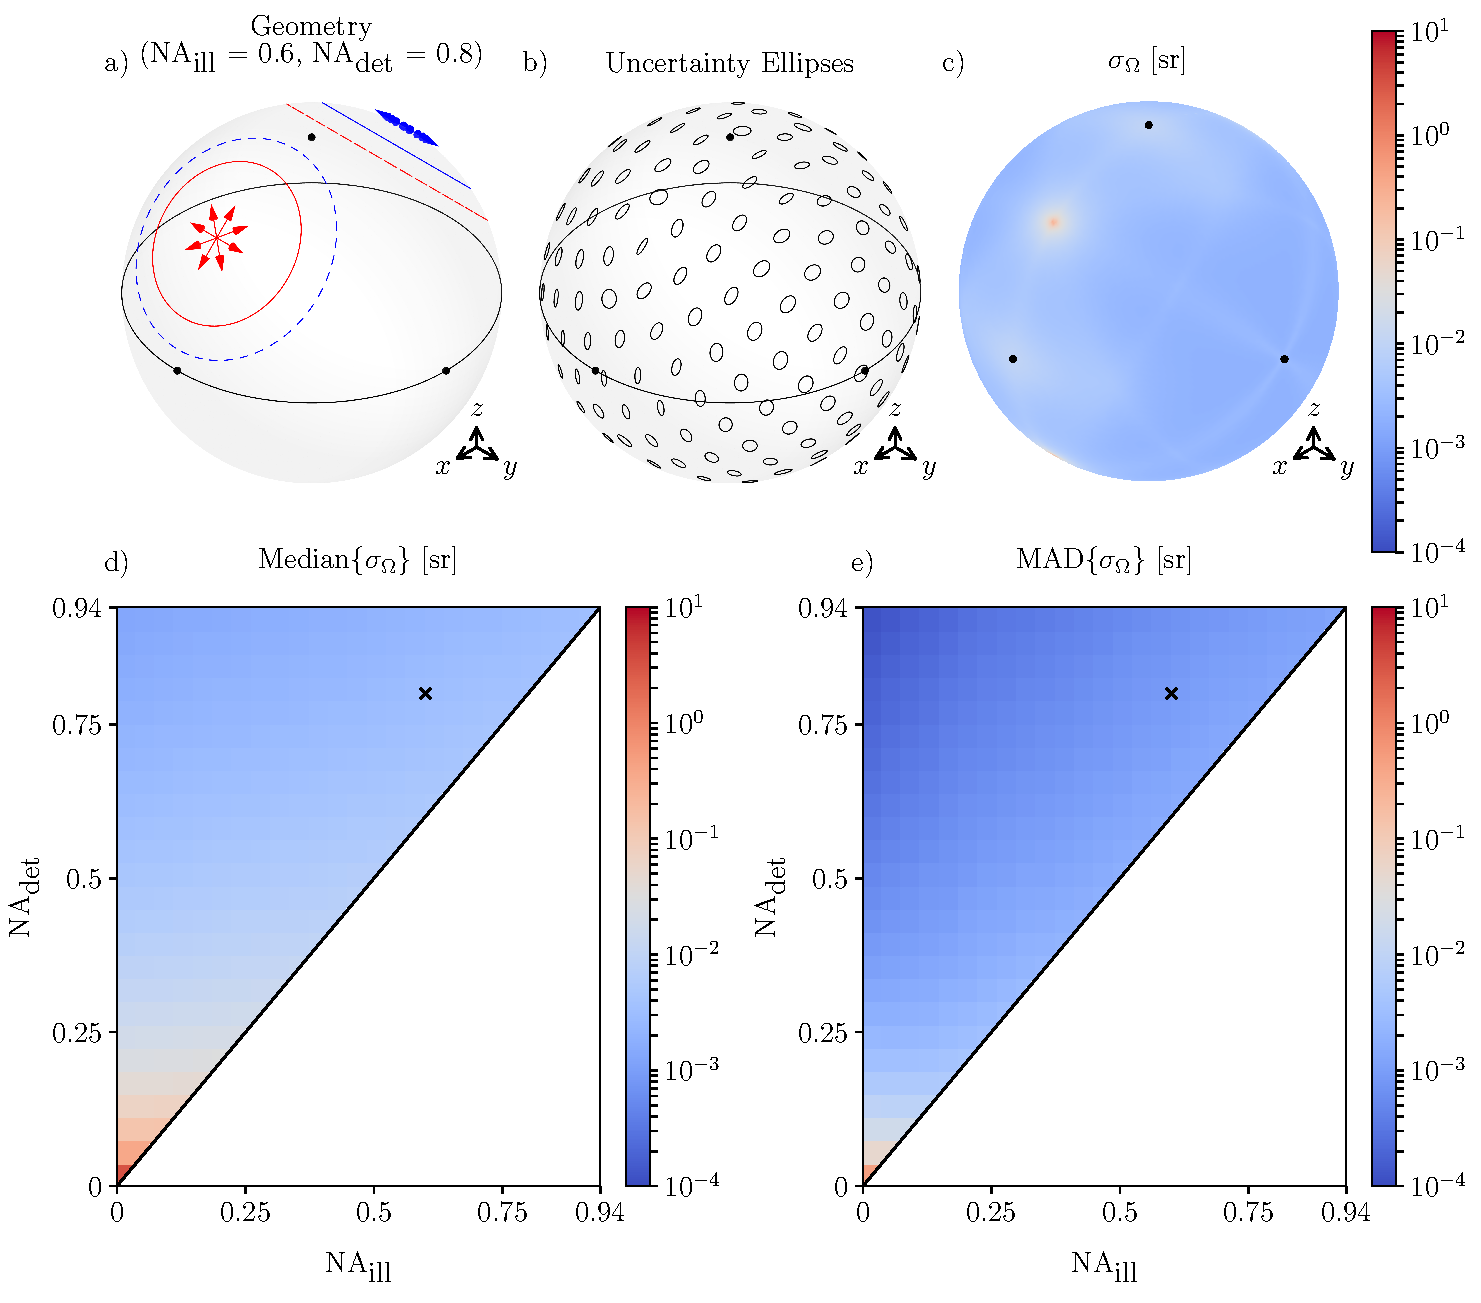
\includegraphics[width=\textwidth]{double-arm}
\caption{Symmetric widefield designs with varying NA and underfilling of the
  back aperture. See the caption for Fig. \ref{fig:single-arm} for an
  explanation of a)-d).}
\label{fig:double-arm}
\end{figure}

\begin{itemize}
\item Figure \ref{fig:asymmetric-double} shows the results when we considered
  asymmetric light-sheet designs. We kept the two arms orthogonal and used light-sheet
  illumination. We swept the NA asymmetry and the dose asymmetry and found that the
  best results occur for symmetric designs. 
\item There is a tradeoff between solid-angle uncertainty median and MAD. You
  can slightly reduce the mean or variance by using an asymmetric design, but
  you pay for it. Reducing the median increases the MAD and vice-versa.
\item The best dual arm microscope design is a symmetric light-sheet
  illumination microscope with the largest possible detection NA.
\end{itemize}

\begin{figure}[htbp]
\centering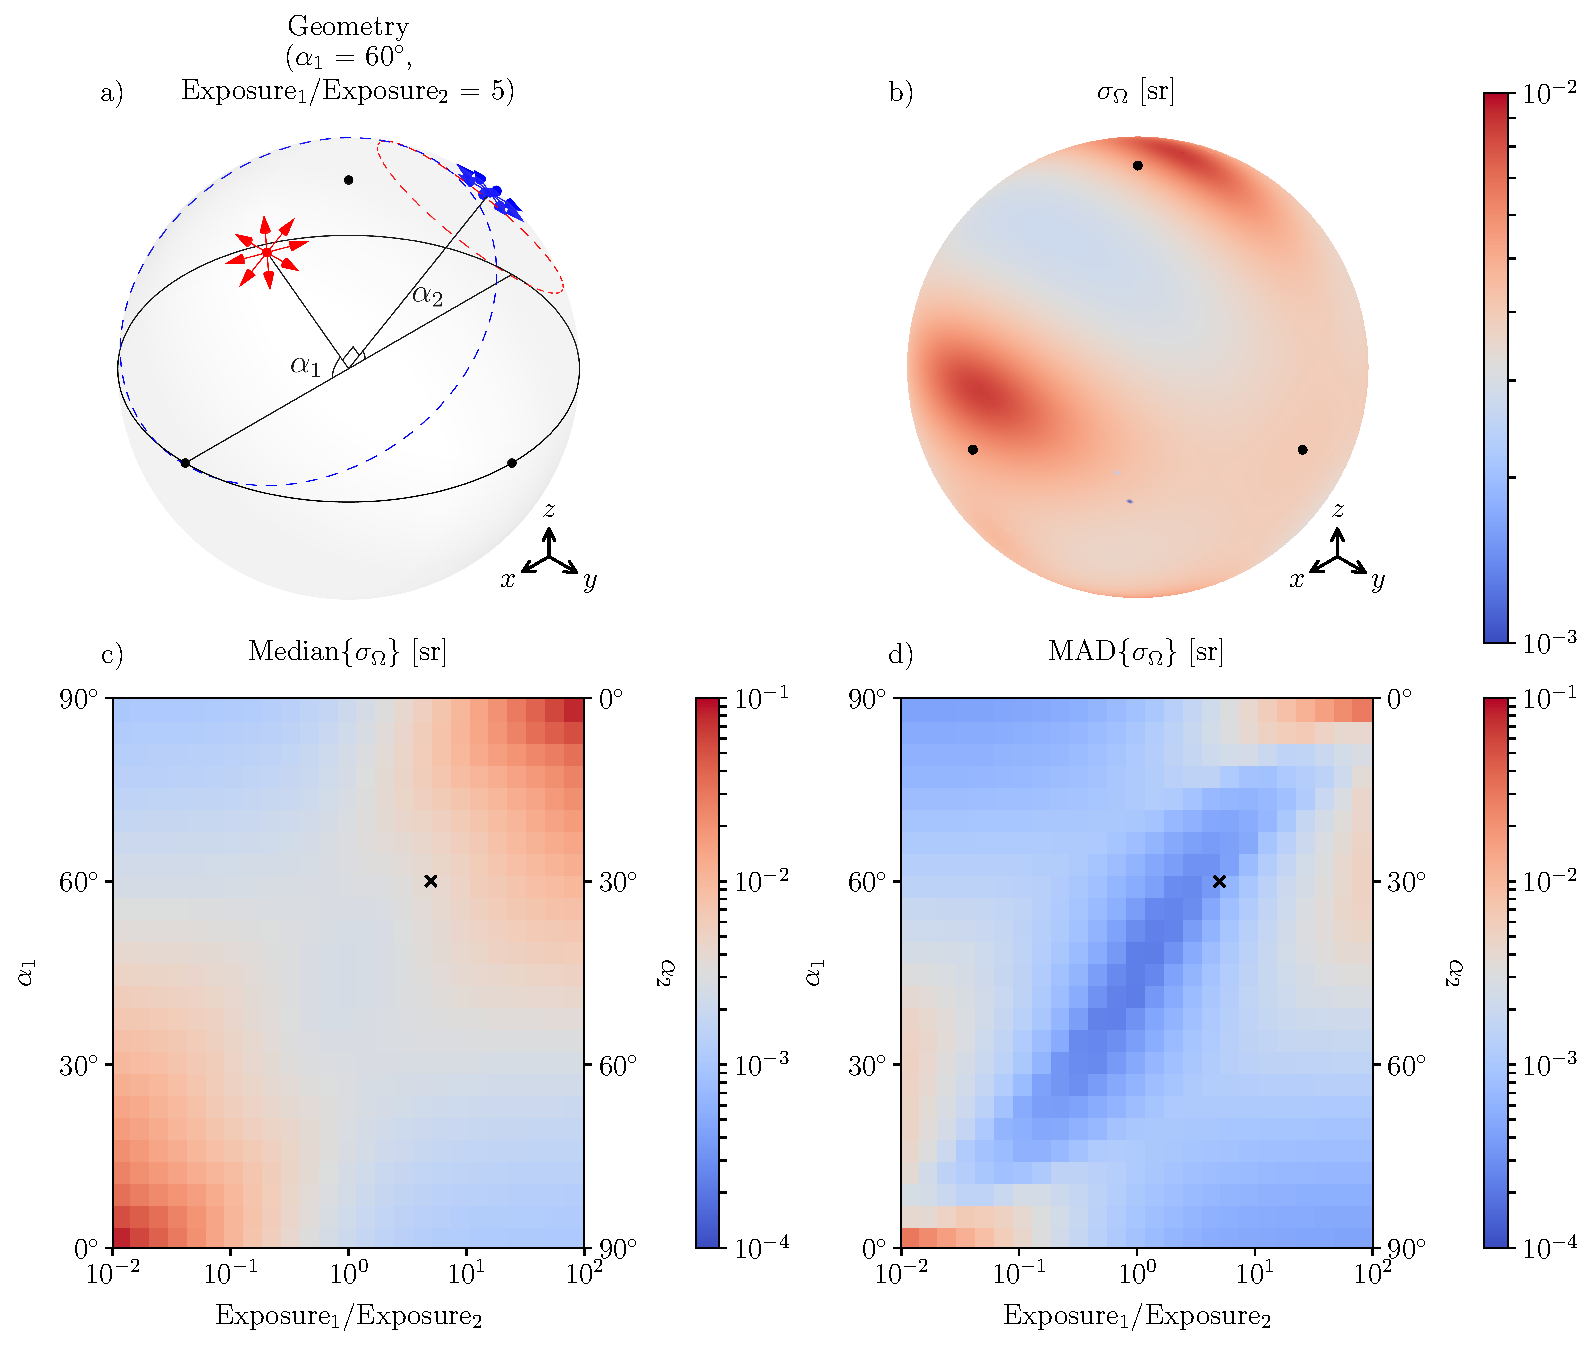
\includegraphics[width=\textwidth]{asymmetric-double}
\caption{Asymmetric light-sheet illumination designs with varying NA and
    dose asymmetry. See the Fig. \ref{fig:single-arm} caption for an explanation of a)-d).}
\label{fig:asymmetric-double}
\end{figure}

\subsection{Three-Arm Designs}
\begin{itemize}
\item Figure \ref{fig:triple-arm} shows the results when we considered
  symmetric light-sheet designs with a lower detection arm. We swept
  through the NA of the upper arms and NA of the lower arm.
\item The results show that the best designs have the largest possible detection
  upper and lower NA.
\item Note to Patrick: I used the same efficiencies for the upper and lower
  arms. I'm still thinking/unsure about the factor of $\sim$1/9 due to rolling
  shutter on the lower objective. If we do end up using this factor it will
  weight the importance of a large NA on the upper objectives.
\item There is a small dip in the MAD when the upper and lower objectives have
  the same NA, but it is still better to use the largest possible lower
  NA. 
\end{itemize}

\begin{figure}[htbp]
\centering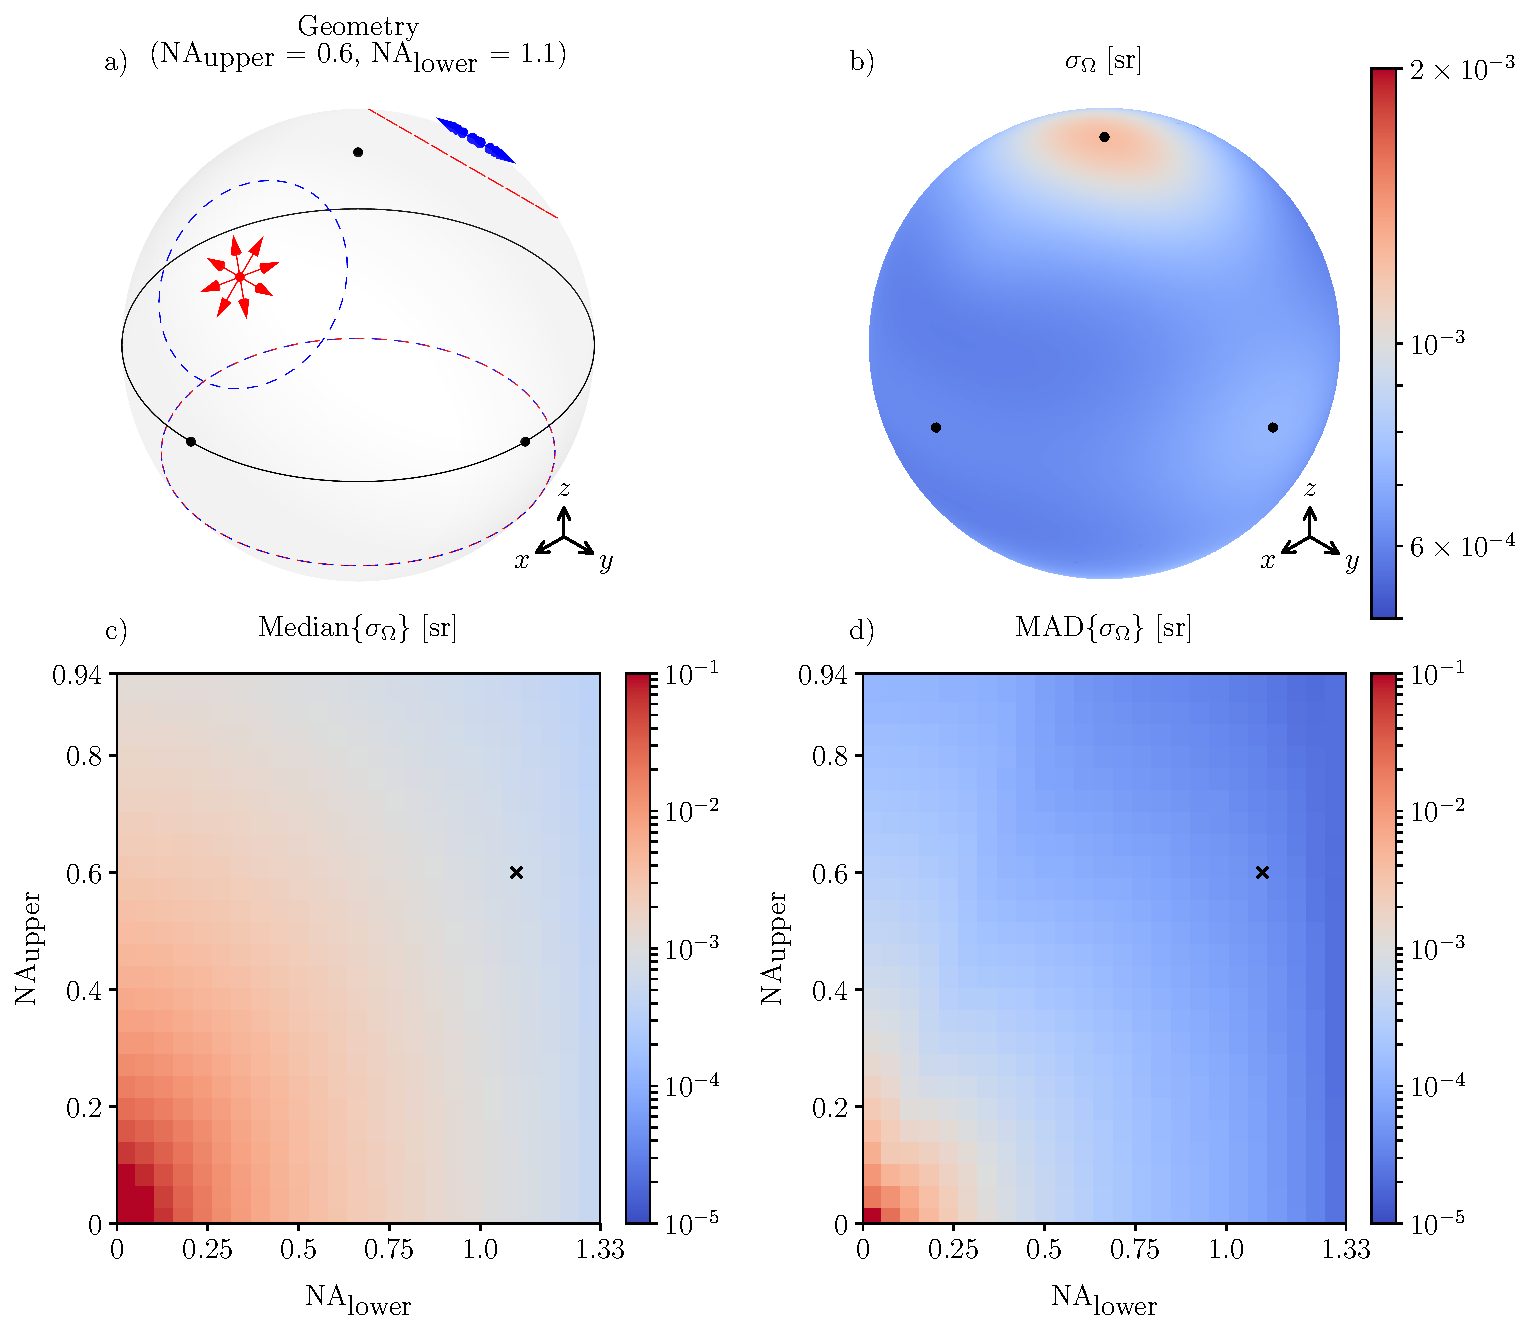
\includegraphics[width=\textwidth]{triple-arm}
\caption{Symmetric light-sheet illumination with lower detection arm and
    varying upper and lower NA. See the Fig. \ref{fig:single-arm} caption for
    an explanation of a)-d).}
\label{fig:triple-arm}
\end{figure}

\section{Discussion}
TODO
% Fourkas' expressions underpredict the fraction of the total power collected by
% an objective with a polarizer by a constant fraction of
% $\frac{3}{2}$. Therefore, using Fourkas' expressions to find $I_{\text{tot}}$
% will result in overpredictions of $I_{\text{tot}}$, but the incorrect
% expressions will not cause any error in the predictions of molecular
% orientation.

% Lu and Bout \cite{lu2008} study the effect of noise on the reconstruction of single fluorophores using Fourkas' expressions. Their main results are unaffected by the correction introduced in these notes, but because these notes predict a higher intensity than Fourkas, Lu and Bout overpredict the effect of noise in their model.

% As noted in \cite{lieb2004}, Fourkas' model only considers single molecules in
% homogeneous environments. 

\section{Conclusion}
TODO

\section*{Funding}
TODO

\section*{Acknowledgments}
TODO
%We thank Hari Shroff and Sean Rose for helpful conversations. 

\section*{Disclosures}
TODO
%The authors declare that there are no conflicts of interest related to this article.

\end{document}
